\chapter{Carrier Recovery}

Carrier recovery is a processes used in coherent demodulation where the phase
and the frequency of the transmitter carrier wave are recovered by the receiver
and thus after having such information it is possible to extract the information
in the transmitted signal.\\
Considering that the phase and frequency of the transmitted wave probably will
be affected by noise, it is not a straight-forward method, it includes filtering
and usually feedback systems to correct the erros in phase or frequency caused
by the noise.\\
This chapter aims in the brief exploration of some techniques used for carrier
recovering, such as Phase locked loops, costas loop and others.\\

\section{Phase-Locked Loop (PLL)}
\label{sec:pll}

Phase-locked Loop is a kind of feedback system, which has been extensively used
in communications sytems and other applications which require frequency
synthesis.\\
The Phase-Locked Loop is composed by three basic components \ref{fig:pll}:

\begin{enumerate}
    \item A phase detector (PD).
    \item A loop filter.
    \item A voltage-controlled oscillator (VCO).
\end{enumerate}

As it can be seen in the figure \ref{fig:pll} the phase-locked loop is a feedback
system whose main goal is to make the output signal the same as the input
signal. Basically the phase detector compares the phase of the input signal
against the phase of the VCO output, then the PD output is inputed in the loop
filter whose output is the voltage that controls the VCO. The output of the
phase detector is the phase error between the input signal and the VCO and the
output of the loop filter outputs the control voltage to the VCO.\\

When the loop is locked, theoretically, the output frequency is the same as the
input frequency, but to maintain the control voltage necessary to lock it is
needed a nonzero output to the phase detector, thus the pll operates with some
phase error, but this tends to be small.\\

Pll makes simple to syntetize frequencies with a pll and do operations
of analog modulation and demodulation, these applications willbe briefly
discussed later.


\begin{figure}[htbp]
    \centering
    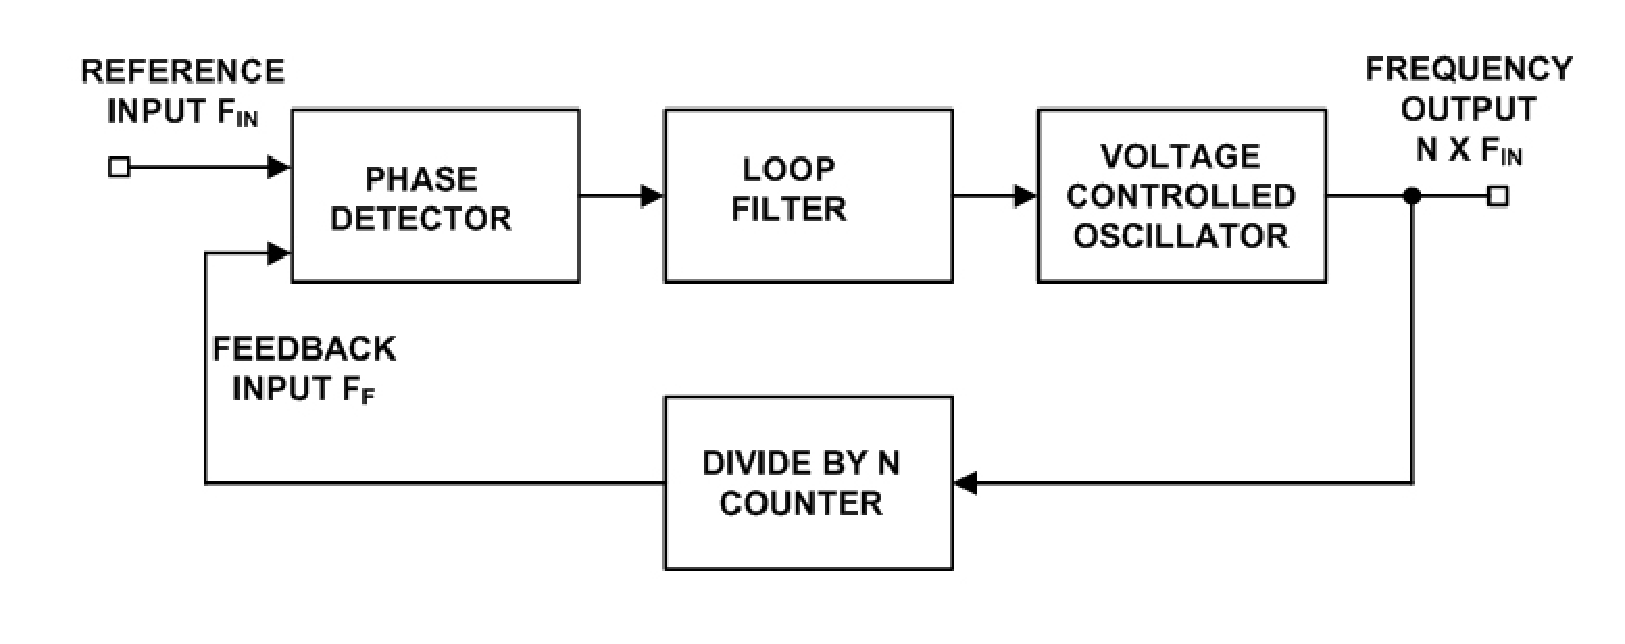
\includegraphics[width=0.65\textwidth]{./figures/pll.eps}
    \caption{ Basic PLL scheme
    \label{fig:pll}}
\end{figure}

\subsection{PLL Fundamentals}
Considering a basic pll scheme as shown in figure \ref{fig:pll2} we can see that
the input signal has a phase of $\theta_i(t)$ and the VCO output has a phase of
$\theta_o(t)$. Assuming that the loop is locked and the phase detector is
linear, the ouput of the PD is proportional to the phase difference between its
inputs, thus,

\begin{equation}
    v_d = K_d(\theta_i - theta_o)
    \label{eq:pdout}
\end{equation}

where $k_d$ is the PD gain factor and its unity is volt/radian.\\

The $v_d$ is filtered by the loop filter, supressing noise and high frequency
signal components, the filter also contributes for the determination of the
dynamic performance of the loop. The filter transfer function is given by
$F(s)$.

Frequency output of the VCO is determined by the input $v_c$ and since frequency
is the derivative of the phase, the operation in the VCO can be described by,

\begin{equation}
    L[\frac{d\theta_o(t)}{dt}] = s\theta_o(s)=K_oV_c(s)
    \label{eq:vco}
\end{equation}

\begin{figure}[htbp]
    \centering
    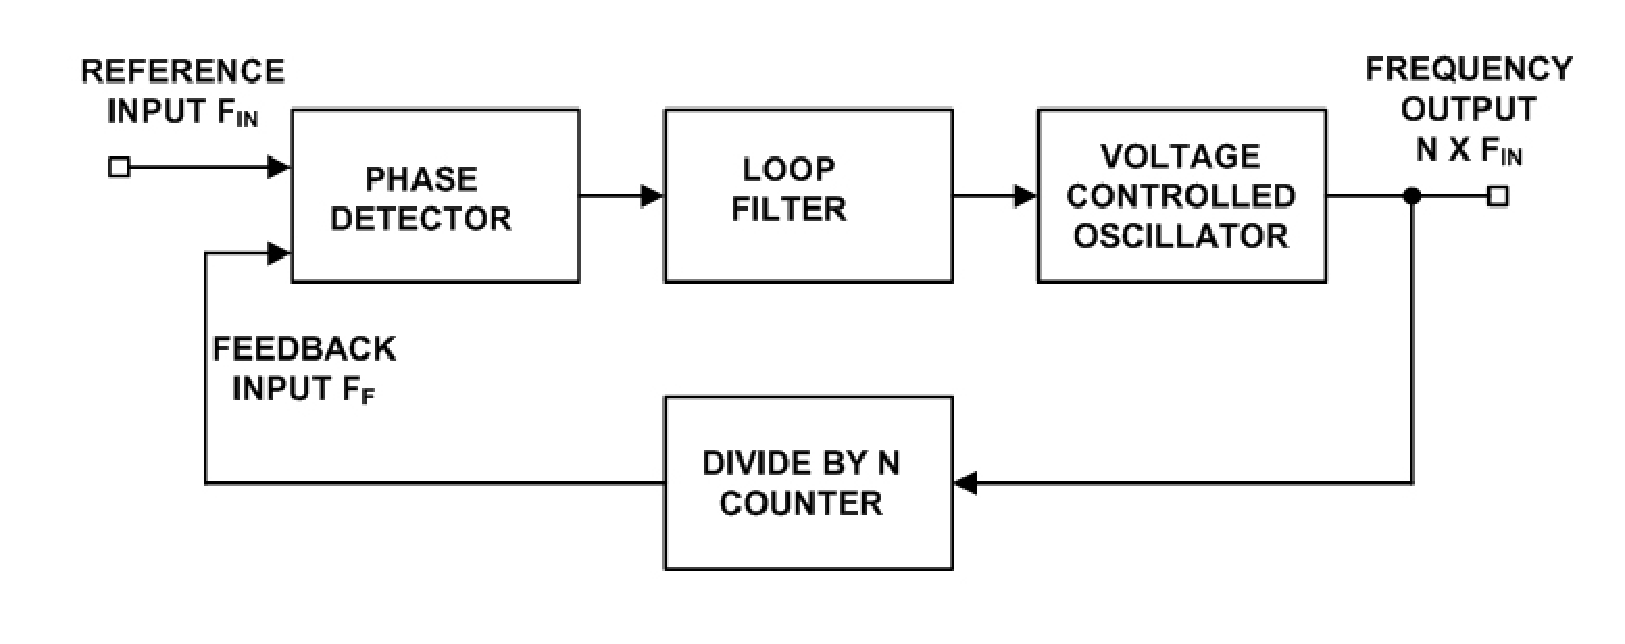
\includegraphics[width=0.65\textwidth]{./figures/pll.eps}
    \caption{ PLL
    \label{fig:pll2}}
\end{figure}

we can see that the output of the VCO is linearly related to the integral of the
control voltage.\\

Using laplace notation it is possible to stablish some basic equations to
describe the loop components behavior,

\begin{equation}
    V_d(s)=K_d[\theta_i(s) - \theta_o(s)]
    \label{eq:vd}
\end{equation}

\begin{equation}
    V_c(s)=F(s)V_d(s)
    \label{eq:vc}
\end{equation}

\begin{equation}
    \theta_o(s)=\frac{k_oV_c(s)}{s}
    \label{eq:thetao}
\end{equation}

The combination of these equations \ref{eq:vd}, \ref{eq:vc}, \ref{eq:thetao}
results in the basic loop equations:


\begin{equation}
    H(s)= \frac{\theta_o(s)}{\theta_i(s)}=
    \frac{K_oK_dF(s)}{s + K_oK_dF(s)}
    \label{eq:gentf}
\end{equation}

\begin{equation}
    \frac{\theta_i(s)-\theta_o(s)}{\theta_i(s)}=
    \frac{\theta_e(s)}{\theta_i(s)}=
    \frac{s}{s+K_oK_dF(s)}=1-H(s)
    \label{eq:pherr}
\end{equation}

\begin{equation}
    V_c(s)=\frac{sK_dF(s)\theta_i(s)}{s+K_oK_dF(s)}=
    \frac{s\theta_i(s)}{K_o}H(s)
    \label{eq:vchs}
\end{equation}

Where:

\begin{itemize}
    \item $H(s)$ is the closed-loop transfer function
    \item $\theta_e$ is the phase error
\end{itemize}

There is indeed another point to explore, regarding loop gain, the open-loop
transfer function (open-loop gain) of any PLL is,

\begin{equation}
    G(s)=\frac{K_oK_dF(s)}{s}
    \label{eq:olg}
\end{equation}

thus the closed-loop transfer function can be made in terms of \ref{eq:olg},

\begin{equation}
    H(s)=\frac{G(s)}{1+G(s)}
    \label{eq:clg}
\end{equation}

The DC gain can be defined as,

\begin{equation}
    K_v=K_oK_dF(0)
    \label{eq:dcgain}
\end{equation}

which has dimensions of frequency ($time^-1$). A high $K_v$ value is related to
a good performance of the loop. $F(s)$ is a rational function of the loop filter
in the form

\begin{equation}
    F(s)=\frac{g(s -z_1)(s-Z_2)\dots(s-z_m)}
    {(s-p_1)(s-p_2)(s-p_3)\dots(s-p_n-1)}
    \label{eq:filterrf}
\end{equation}

For the filter to be realizable m cannot exceed n-1, and if m=n-1 as often
occurs in PLL designs, then $g=F(\infty)$.

Expandign $F(s)$ in aprtial fractions it is possible to rewrite the open-loop
gain function as

\begin{equation}
    G(s)=\frac{K}{s}\Bigg[ a_1+\sum_{i=1}^{n-1} \frac{a_i+1}{s-p_i}\Bigg]
    \label{eq:gsfilter}
\end{equation}

where $K$ is the $loop gain$  and $a_1$ is zero if $m < n-1$, while $a_1 = 1$ 
if $m = n-1$, but K is only "defined" when $a_1 = 1$, thus the most important
PLLs are designed for $a_1 = 1$ (equal number of poles and zeroes in the loop
filter).

Based on the previous equations which describe the behavior of the components in the
phase-locked loop we can classify the pll based on the order of the transfer
function associated with the loop. This classification is based upon the nunmber
of perfect integrators ($\frac{1}{s}$) present in the transfer function.

\begin{itemize}
    \item First order loop.
    \item Second order loop.
    \item Third and higher order loop.
\end{itemize}

\subsubsection{First Order Loop}

The first order loop is the simplest implementation of a phase-locked loop,
where the loop filter is ommited, thus $F(s)=1$

\begin{equation}
    H(s)= \frac{K_oK_d}{s + K_oK_d}=
    \frac{K}{s + K}
    \label{eq:tf1st}
\end{equation}

Where:
\begin{itemize}
    \item $K = K_oK_d =K_v$;
\end{itemize}

In the first-order loop the only parameter avaible to the designer is the loop
gain

\subsubsection{Second Order Loop}

In the second order loop the loop filter is used and it is possible to separate
it in two major "classes", the loop which use passive filters and the loops
whose use active filters. The loops which use passivel filters require high-gain
DC amplifier but provides good tracking performance, the closed-loop transfer
function for a passive filter is

\begin{equation}
    H_1(s)=\frac{K_oK_d(s\tau_2+1)/\tau_1}
    {s^2+s(1+K_oK_d\tau_2)/\tau_1+K_oK_d/\tau_1}
    \label{eq:tf2ndpass}
\end{equation}

and for rthe active filter the closed-loop trasnfer function is

\begin{equation}
    H_2(s)= \frac{K_oK_d(s\tau_2+1)/\tau_1}
    {s^2+s(1+K_oK_d\tau_2)/\tau_1+K_oK_d/\tau_1}
    \label{eq:tf2ndact}
\end{equation}

witha very large amplifier gain \ref{eq:tf2ndpass} and \ref{tf2ndact} can be 
rewritten as

\begin{equation}
    H_1(s)= \frac{s(2\zeta\omega_n-\omega_n^2/K_oK_d)+\omega_n^2}
    {s^2+2\zeta\omega_ns+\omega_n^2}
    \label{eq:damph1}
\end{equation}

\begin{equation}
    H_1(s)= \frac{2\zeta\omega_ns+\omega_n^2}
    {s^2+2\zeta\omega_ns+\omega_n^2}
    \label{eq:damph2}
\end{equation}

where $\omega_n$ is the natural frequency of the loop and $\zeta$ is the damping
factor.\\

The second-order loops are the most prevalent used loop but depending on the
application another loop orders are required.

\subsubsection{Third Order Loops}

As stated before, depending on the situation the third-order loop is necessary
because it can track a frequency ramp with zero steady error for example. The
basic setup of a third order PLL is when the two poles of the filter are at the
origin, that is, if the loop filter has two cascated integrators, so the closed
loop transfer function is

\begin{equation}
    H(s)=\frac{K(s^2+a_2s+a_3)}{s^3+K(s^2+a_2s+a_3)}
    \label{eq:tf3rd}
\end{equation}

it is rare to see a loop built with an order higher than 3, because as the order
raises the more difficult it is to stabilize the loop and it gets more sensitive
to to changes in the gain circuit components.

\subsubsection{Analysis Tools}
There are two main ways to analyse the behavior of a phase-locked loop one of
them is the root-locus plot which can be built by determining the locations of
the poles of the closed-loop response, these poles change their location as the
gain is changed throught the s-plane. The root-locus plot is used to show these
paths and can be easily obtained by following a few simple rules.(appendice root
locus)

\begin{figure}[htbp]
    \centering
    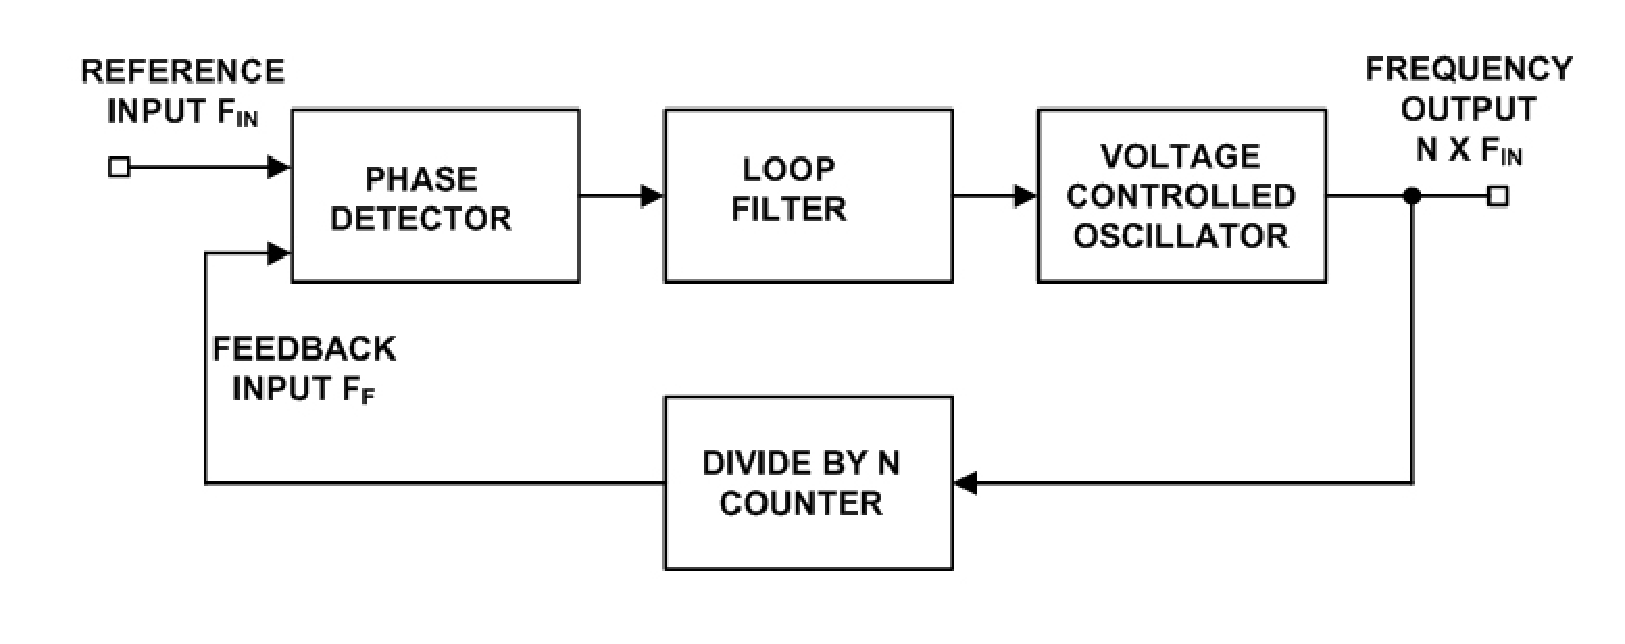
\includegraphics[width=0.65\textwidth]{./figures/pll.eps}
    \caption{ Root-Locus plot for a first-order PLL
    \label{fig:rlocus1}}
\end{figure}

\begin{figure}[htbp]
    \centering
    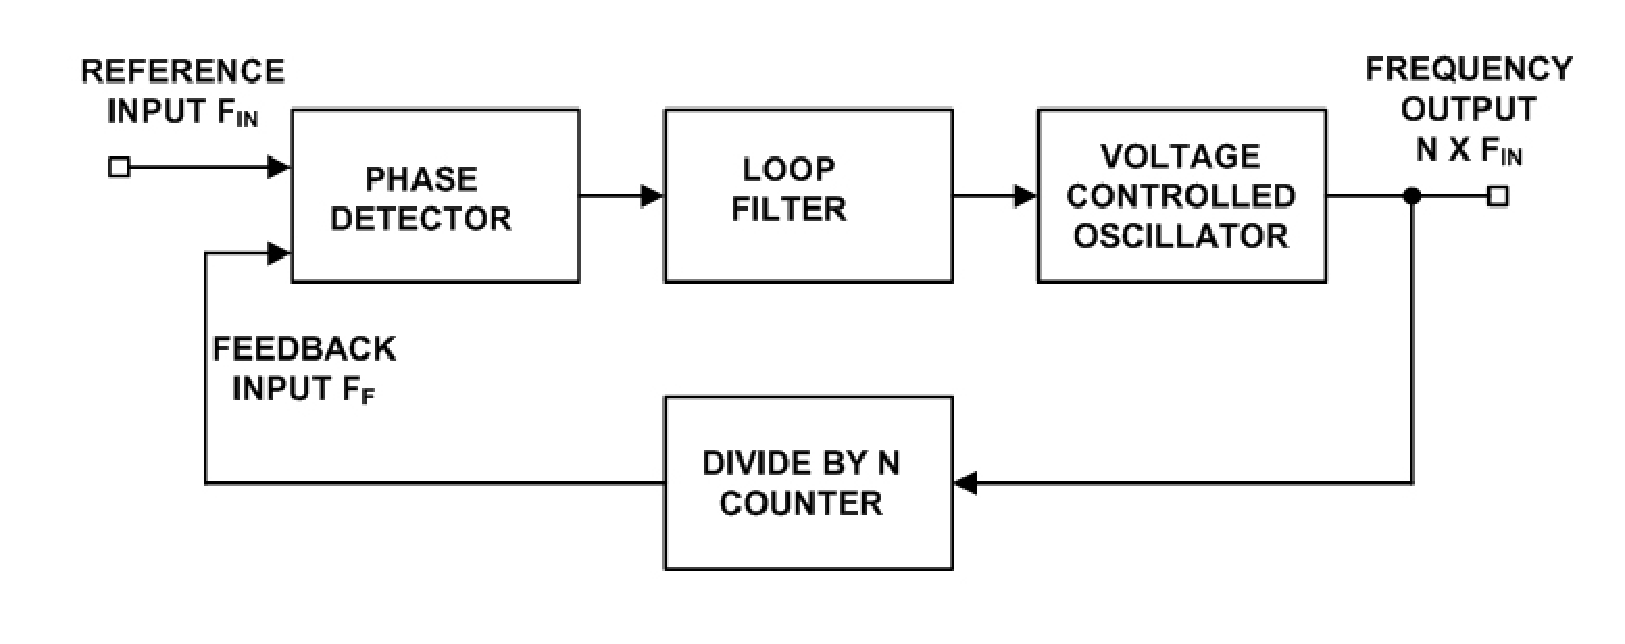
\includegraphics[width=0.65\textwidth]{./figures/pll.eps}
    \caption{ Root-Locus plot for a second-order PLL
    \label{fig:rlocus2}}
\end{figure}

\begin{figure}[htbp]
    \centering
    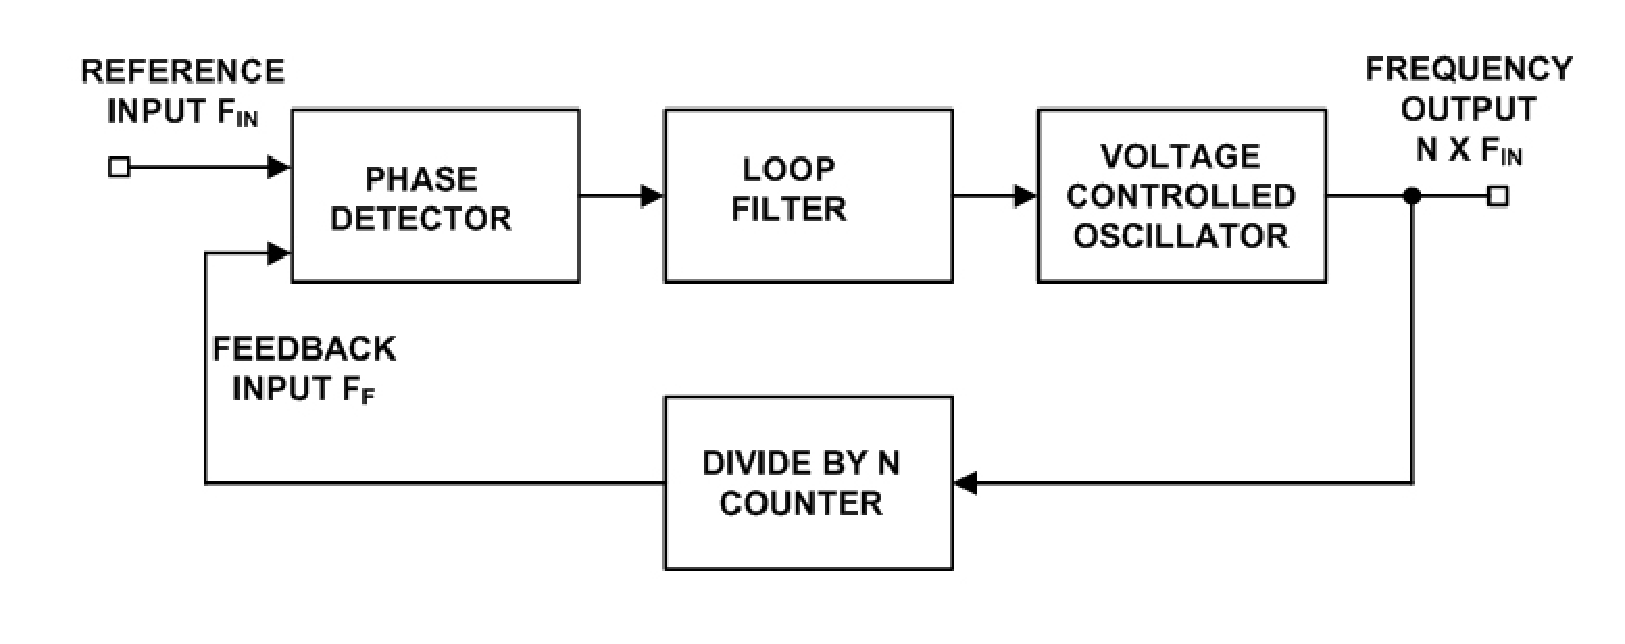
\includegraphics[width=0.65\textwidth]{./figures/pll.eps}
    \caption{ Root-Locus plot for a third-order PLL
    \label{fig:rlocus3}}
\end{figure}

Another useful tool is the Bode plot (apendice bode plot), which is a pair of
curves displaying the polar components of $G(j\omega)$.

\begin{figure}[htbp]
    \centering
    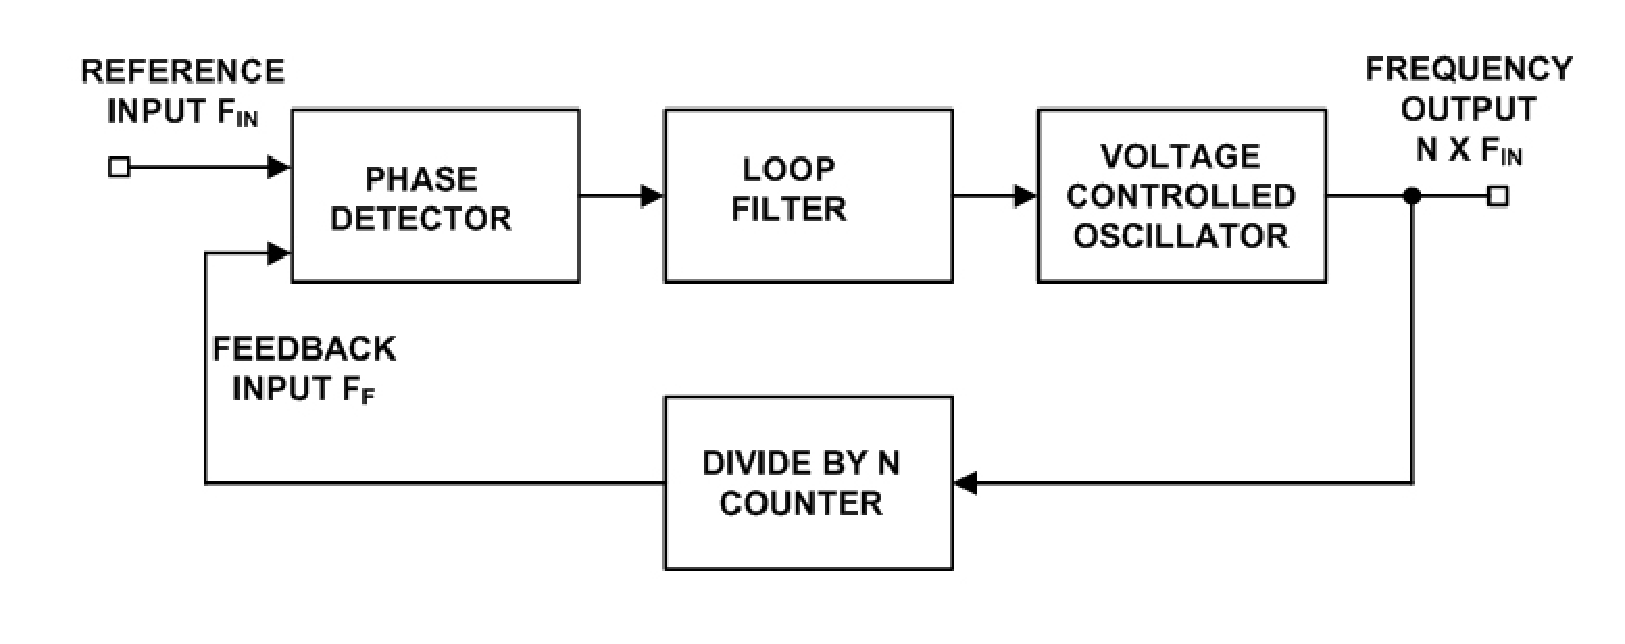
\includegraphics[width=0.65\textwidth]{./figures/pll.eps}
    \caption{ Root-Locus plot for a third-order PLL
    \label{fig:rlocus3}}
\end{figure}

\begin{figure}[htbp]
    \centering
    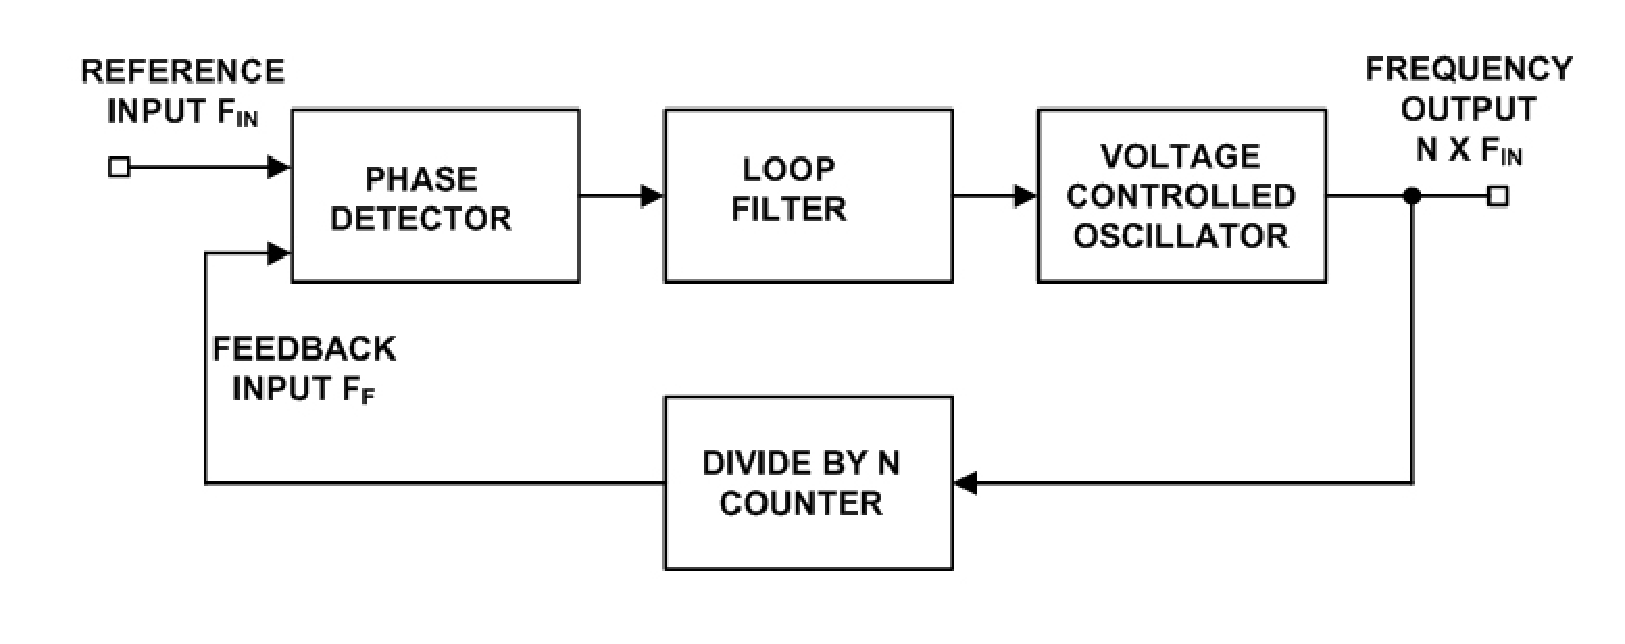
\includegraphics[width=0.65\textwidth]{./figures/pll.eps}
    \caption{ Root-Locus plot for a third-order PLL
    \label{fig:rlocus3}}
\end{figure}

\begin{figure}[htbp]
    \centering
    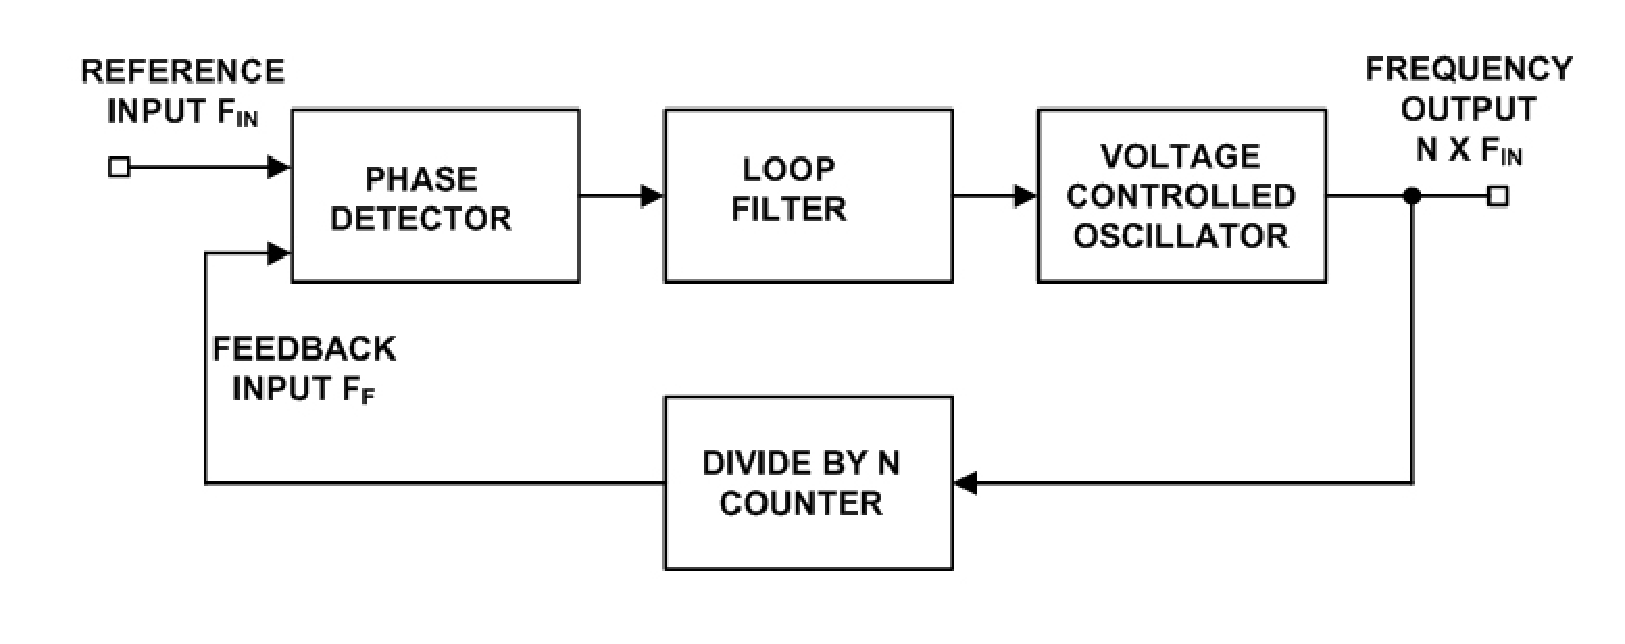
\includegraphics[width=0.65\textwidth]{./figures/pll.eps}
    \caption{ Root-Locus plot for a third-order PLL
    \label{fig:rlocus3}}
\end{figure}

\begin{figure}[htbp]
    \centering
    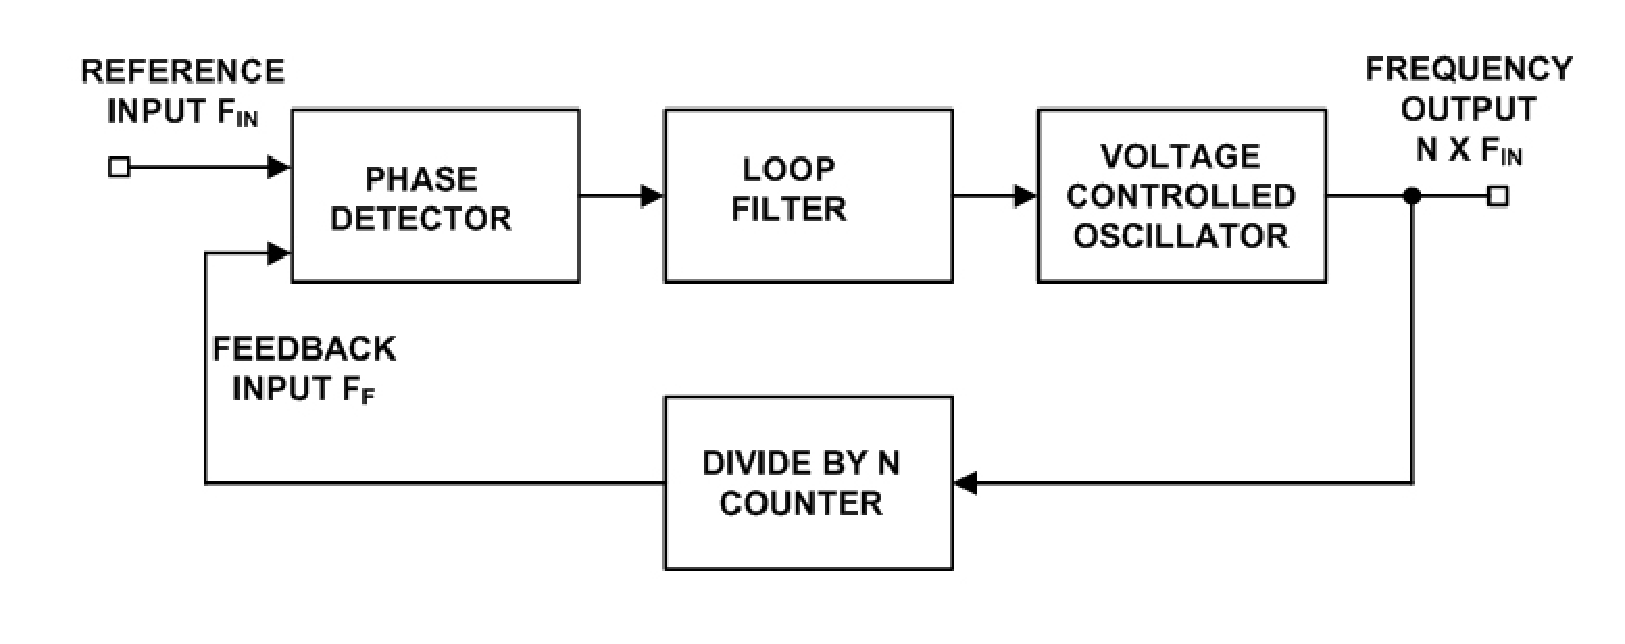
\includegraphics[width=0.65\textwidth]{./figures/pll.eps}
    \caption{ Root-Locus plot for a third-order PLL
    \label{fig:rlocus3}}
\end{figure}

\subsection{PLL Components}
As stated in the beginning of this section and as can be seen in the figure
\ref{fig:pll} the elementary Phase-locked Loop is composed of three main 
components, the phase detector, the loop filter and the voltage-controlled 
oscillator. This subsection aims in introducting the basic components and any
useful theory.

\subsubsection{Loop Filter}

\subsubsection{Voltage-Controlled Oscillator}

\subsubsection{Phase-Detector}

\subsection{Linearized Analogic PLL Tracking}
Since the scope of this work is not PLL itself the nonlinear behavior will not
be explored here, all the assumptions in this subsection shall be of linearized
loops.\\
To understand tracking it is necessary to understand the PLL behavior until it
locks and consequently the noise behavior of the PLL is also an important
matter.\\
\subsubsection{Noise Behavior}


\subsection{Modulation and Demodulation using PLL}

\subsection{Discrete-time PLL}

\subsection{Design of PLL and DPLL}

\subsection{Costas Loop}

